Figure \ref{fig:re-papr} investigates the relationship between PAPR and R-E region for $N = 8, 16$ under the FF and FS channel response as in Figure \ref{fig:siso-channels}.

\begin{figure}[ht]
  \centering
  \subfigure[FF: $N = 8$]{
    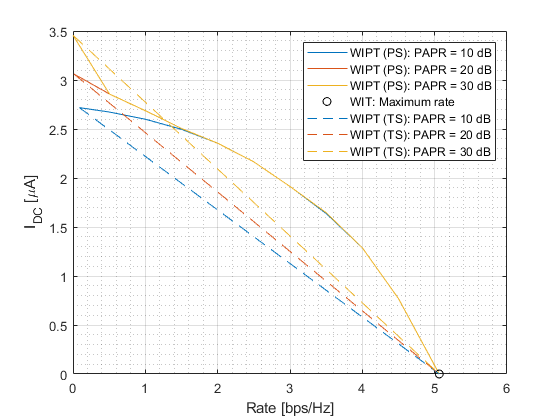
\includegraphics[width=0.48\textwidth]{siso_re_ff_papr_8}\label{fig:re-ff-papr-8}}
  \subfigure[FF: $N = 16$]{
    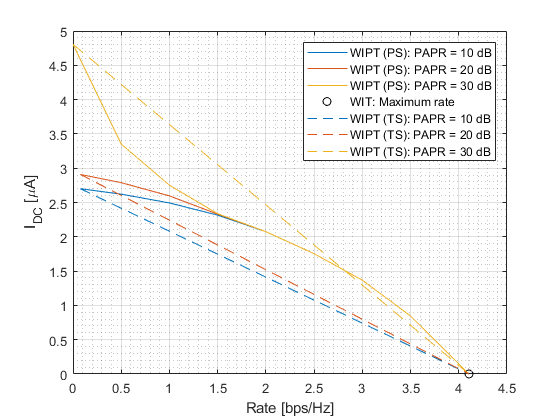
\includegraphics[width=0.48\textwidth]{siso_re_ff_papr_16}\label{fig:re-ff-papr-16}}
  \quad
  \subfigure[FS: $N = 8$]{
    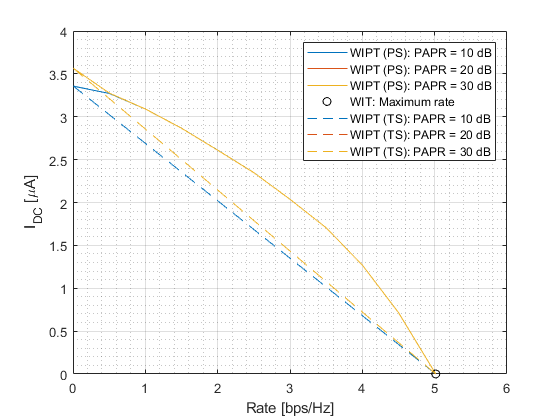
\includegraphics[width=0.48\textwidth]{siso_re_fs_papr_8}\label{fig:re-fs-papr-8}}
  \subfigure[FS: $N = 16$]{
    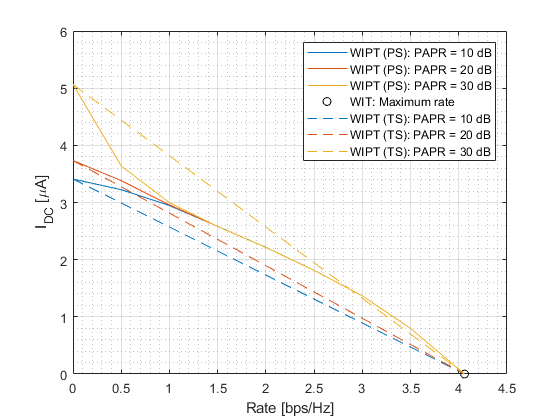
\includegraphics[width=0.48\textwidth]{siso_re_fs_papr_16}\label{fig:re-fs-papr-16}}
  \caption{R-E region vs PAPR for FF channel}
  \label{fig:re-papr}
\end{figure}

A first observation is that a large enough PAPR is required to fully exploit the power gain of the multisine waveform. For $N = 16$, the R-E region is convex for a PAPR no larger than 20 dB and is concave-convex when it increases to 30 dB. Compare the result with Figure \ref{fig:snr-ff-20db}} and \ref{fig:snr-fs-20db}}, it can be observed that with a small PAPR constraint of 10 dB, the use of multisine waveform is strictly restricted such that the modulated waveform dominates the transmit signal. Hence, the corresponding R-E plot is similar to the result without power waveform. On the contrary, a PAPR of 30 dB is large enough for the optimal performance of the superposed signal in the low-rate region. It can be concluded that the energy benefit of the multisine waveform indeed comes from the high PAPR. In each cycle, the pulse-like peak pushes the rectifier output voltage to a high level which decreases slowly in the rest of the period.

A contrast of the R-E region achieved by $N = 8$ and 16 also suggests a larger $N$ requires higher PAPR for the optimal performance. This verifies the discussion in section \ref{sec:rectenna-behavior} and further suggests that although increasing $N$ can effectively boost the harvested energy, the PAPR constraint may limit the use of a very large $N$ in practice. 